\documentclass[a4paper]{article}
\usepackage{interspeech2012,amssymb,amsmath,graphicx}
\usepackage{algorithm}
\usepackage{algorithmic}
\usepackage{mathtools}
\usepackage{graphicx}
\usepackage{tabularx}
\usepackage{flushend} % for even columns on last page
\sloppy	% better line breaks

%for dot/graphviz
\usepackage{tikz}
\usetikzlibrary{snakes,arrows,shapes}
\ninept	% optional



%\title{An Adaptive Emotional Questioner Agent using Bayesian Belief Update}
\title{A Sequential Bayesian Dialog Agent for Computational Ethnography}


\makeatletter
\def\name#1{\gdef\@name{#1\\}}
\makeatother
%\name{{\em Abe Kazemzadeh}}
\name{{\em Abe Kazemzadeh, James Gibson, Juanchen Li, Sungbok Lee,}\\ {\em Panayiotis Georgiou, Shrikanth Narayanan}}

\address{
Signal Analysis and Interpretation Lab, University of Southern California\\
Los Angeles, CA, USA \\
{\small \tt \{kazemzad@,jjgibson@,juanchel@,sungbokl@,georgiou@sipi.,shri@sipi.\}usc.edu}}


%\newcommand{\argmax}[1]{\underset{#1}{\operatorname{argmax}}}

\begin{document}
\maketitle


\begin{abstract}
{%\ninept
We present a sequential Bayesian belief update algorithm for an emotional
dialog agent's inference and behavior.  This agent's purpose is to collect
usage patterns of natural language description of emotions among a community
of speakers, a task which can be seen as a type of computational ethnography.
We describe our target application, an emotionally-intelligent agent that can
ask questions and learn about emotions through playing the emotion twenty
questions (EMO20Q) game.  We formalize the agent's algorithms mathematically
and algorithmically and test our model experimentally in an experiment of 45
human-computer dialogs with a range of emotional words as the independent
variable. We found that 44\% of these human-computer dialog games are
completed successfully, in comparison with earlier work in which human-human
dialogs resulted in 85\% successful completion on average.  Despite being
lower than this upper-bound of human performance, especially on difficult
emotion words, the subjects rated that the agent's humanity was 6.1 on a 0 to
10 scale. This indicates that the algorithm we present produces realistic
behavior, but that issues of data sparsity may remain.
}
\end{abstract}
\noindent{\bf Index Terms}: dialog agents, emotion recognition, chatbot,
EMO20Q, 


\section{Introduction}

The evolution of language in our primitive ancestors endowed early humans with
the ability to communicate about things beyond their immediate perception. In
addition to feeling and expressing emotions in response to current situations
\cite{Marsella2009}, we are also able to talk about emotions that may have
occurred in the past or that may be altogether hypothetical.  Non-human
primates and many other animals can display their emotions through social
signals, but only humans can communicate about their emotions symbolically.

Some aspects of human emotions are social signals, e.g. facial features, that
show stability across cultures and even across species.  However, some key
aspects of emotional behavior in humans is symbolic: the words that designate
emotions in natural languages are conventional symbols.  The relation of
emotions as social and biological signals with the symbolic processes of
natural language is what we call {\em natural language description of emotions}.

Whereas humans have both emotions and the ability to manipulate symbols using
language, computers are only able to manipulate symbols and lack biological
emotion pathways.  To what extent these biological processes of emotion affect
natural language description of emotion, and to what extent this language can
be learned and simulated by an ``emotionless'' computer, is currently an open
question and the topic of this paper.

In the field of affective computing, it is common to rely on a limited set of
basic emotions to be used for labeling emotional data.  However, when
considering natural language descriptions of emotions there are a practically
limitless number of ways to name and describe emotions.  As long as a
community of speakers decides, by customs or convention, to designate an
emotion using an arbitrary sequence of phonemes (c.f. {\em duality of
  patterning} \cite{Hockett1968}) , we must, at some point, deal with emotion
labels that cannot be simply enumerated theoretically.  Instead, we propose an
agent that will carry out the laborious task of eliciting natural language
descriptions of emotion in the populations that we wish to study.  We feel
that this elicitation process can be thought of as a type of computational
ethnography \cite{Arnold2010} for a linguistic community of practice
\cite{Wenger1998}.

In previous work \cite{Kazemzadeh2011a}, we collected natural language
descriptions of emotions from a target population using a game called emotion
twenty questions (EMO20Q), which is the familiar game of twenty questions
played with emotions as the unknown objects.  Based on the data we collected
of humans playing EMO20Q, we created a statistical model for an agent who
plays EMO20Q using a sequential Bayesian update algorithm.  This algorithm can
be seen as a simplification of the partially observable Markov decision
process for dialog systems \cite{Williams2007,Thomson2008}.  The
simplification is made possible due to the constrained interaction of the
twenty questions task. For elicitation of human knowledge, the goal for our
agent is to play realistically and to approach human performance in
successfully completing the EMO20Q task.  The data we used for training and
testing is described in Section~\ref{sec:data}.  The model, algorithm, and
implementation for our agent is described in \ref{sec:methodology} and the
results are presented in Section~\ref{sec:results} and discussed in
Section~\ref{sec:discussion}.


%\vspace{-10pt}

\section{Data}
\label{sec:data}
We trained our agent on data from both human-human and human-computer EMO20Q
matches.  A match in the context of EMO20Q is a game-instance where one player
assumes the role of the answerer and the other player, the role of the
questioner.  Typically, in the human-human matches, the players will
alternately switch roles.  In the case of human-computer matches, the computer
always plays the questioner role.

Using the methodology described in \cite{Kazemzadeh2011a}, we collected 110
human-human dialogs, and using an earlier version of our system
\cite{Kazemzadeh2011d}, we collected 131 human-computer dialogs.  In the 110
matches that we collected between two humans, we found that the matches where
the target emotion word was guessed 85\% of the time after approximately 11.4
turns.  In the early versions of the dialog agent, not those described in the
current paper, the performance was much lower than the human-human case.
However, due to using a computer agent, we were able to collect more data with
less effort because the agent was available to play online.

Our current system is an offline desktop application that has an asynchronous
chat-based design and a new algorithm, described in the next section.
To test our algorithm we collected a new set of data using the implementation
of the new algorithm.  The 15 subjects were told that they would play EMO20Q
with a computer and they were asked to pick 3 emotion words, one easy word,
one medium word, and one difficult one, based on how difficult they thought it
would be to guess.  They were also asked to rate the naturalness of the agent
on a 0-10 scale, and were given an opportunity for open-ended comments.

%\vspace{-10pt}

\section{Methodology}
\label{sec:methodology}
\subsection{Framework for Sequential Bayesian Belief Update}

%% %%some of this could be moved to medthod 



%Then it sequentially
%% asks questions and builds a feature vector out of question-answer pairs.  At
%% each iteration the agent chooses the question that is most likely to give an
%% `informative' answer given the current emotion model.  It then updates the
%% posterior probability of the emotions according to according to Bayes rule,
%% utilizing the observed question-answer features from all the question asked.
%% To evaluate the realism of the agent, we experimentally compare its
%% performance to human performance and we also collect qualitative judgments
%% from the experimental subjects.  Moreover, the data generated by testing the
%% agent can be used as more ethnographic training data.


The model we use for the agent is a sequential Bayesian belief update
algorithm that starts with a conditional probability distribution estimated
from a corpus of human-human and human-computer EMO20Q matches, as described
in Section \ref{sec:data}. In this data, there was a set of 105 emotion words
that were observed.  Let $E$ be this set of 105 emotion words and let
$\varepsilon \in E$ be a categorical, Bayesian (i.e., unobserved) random
variable distributed over this set. Each question-answer pair from the match
of EMO20Q is considered as an observed feature of the emotion being predicted.
Thus, if $Q$ is the set of questions and $A$ is the set of answers, then a
question $q \in Q$ and an answer $a \in A$ together compose the feature
$f=(q,a)$, where $f \in Q \times A$. The conditional probability distribution,
$P(f|\varepsilon)$, is estimated from the training data using a smoothing
factor of 0.5 to deal with sparsity.

%% \begin{equation}
%% A = \left\{ 
%%   \begin{array}{l}
%%  \textrm{`yes'} \\  \textrm{`no'} \\  \textrm{`other'} \\  \textrm{`none'} 
%%  \end{array} \right\}.
%% \end{equation} 

In our model we stipulate that the set of answers $A$ are four discrete cases:
``yes'', ``no'', ``other'', and ``none''.  When the answer either contains
forms of `yes' or `no', it is labeled accordingly.  Otherwise it is labeled
`other'.  The forms of `yes' are `yes', `yeah', `yea', `yep', and
`aye'\footnote{These forms of `yes' and `no' were determined from the data.
  The case of `aye' is an example of how some users have tried trick the
  agent, in this case by talking like a pirate.  From the agent's point of
  view, it will be difficult to distinguish the language of population that
  actually includes pirate demographics from language containing experimental
  artifacts like this.  }, and the forms of `no' are `no' and `nope'. The
feature value `none' is assigned to all the questions that were not asked in a
given dialog.  `None' can be seen as a missing feature when the absence of a
feature may be important.  For example, the fact that a certain question was
not asked about a particular emotion may be due to the fact that that question
was not relevant at a given point in a dialog.



%% updates the posterior belief of the  unknown emotion with each answer given in
%% response  to  a  question in  EMO20Q.   In  this  model the  observations  are
%% question-answer pairs  and the hidden  state variable is the  unknown emotion.


Similarly, we stipulate that the questions can be classified into some
discrete class that is specified through a semantic expression as described in
\cite{Kazemzadeh2011a}.  For example, the question ``is it a positive
emotion?'' is represented as the semantic expression ``e.valence==positive''.
If the answer to this question was ``maybe'', the resulting feature would be
represented as {\small \verb#(`e.valence==positive',`other')# }.  

Using Bayes' rule and the independence assumption of the na\"{i}ve Bayes model,
we can formulate the agent's belief about the emotion vector $\varepsilon$
after observing features $f_1 ... f_t$ as
%\vspace{-5pt}
\begin{equation}
\label{naivebayes}
\begin{split}
  P(\varepsilon|f_1,...,f_t) =  &\frac{  \prod_{i=1}^t \left[ P( f_i|\varepsilon) \right]  P(\varepsilon)}{\prod_{i=1}^t P(f_i)} .
\end{split}
%\vspace{-5pt}
\end{equation}

%The most likely emotion is computed according
%to its posterior probability using the Naive Bayes assumption of conditional
%independence in the likelihood:

 %The emotions being guessed by the agent are 



When the game begins the agent can start with a uniform prior on its belief of
which emotion is likely or it can use information obtained in previously
played games.  In the experiment of this paper, we use a uniform prior,
$P(\varepsilon=e_k) =1/|E|, \thickspace \forall k=1...|E|$.  We chose to use
the uniform prior to start with because our training data contains many single
count training instances and because we want to examine how the system
performs with less constraints.  

In (\ref{naivebayes}), the posterior belief of the agent of emotion $e_k$ at time $t$, $P(\varepsilon=e_k | f_1,...,f_t)$ is computed only after the agent has asked the $t$ questions.  In
contrast the formulation we use is dynamic in that the agent updates its
belief at each time point based on the posterior probability of the previous
step, i.e., at time $t$:
%\vspace{-5pt}
\begin{equation}\label{adaptive}
\begin{aligned}
P(\varepsilon|f_1,...,f_t) =&  \frac{  P( f_t|\varepsilon)  P(\varepsilon|f_1,...,f_{t-1})}{P(f_t)} \\
%P(\varepsilon_t|f_1,...,f_t) =&  \frac{  \prod_{i=1}^t \left[ P( f_i|\varepsilon) \right]  P_t(\varepsilon)}{P(f_1,...,f_t)} \\
%P_t(\varepsilon) =&  P_{t-1}(\varepsilon|f_1,...,f_{t-1}) \\
%P_0(\varepsilon) =&  1/|E| .
\end{aligned}
%\vspace{-5pt}
\end{equation}
We introduce a new variable $\beta_{t,k}=P(\varepsilon=e_k | f_1,...,f_t)$
for the agent's belief about emotion $k$ at time $t$ and postulate that the
agent's current prior belief is the posterior belief of the previous
step. Then, the agent's belief unfolds according to the formula:
%\vspace{-5pt}
\begin{equation}\label{adaptive2}
\begin{aligned}
\beta_{0,k} &= P(\varepsilon=e_k) = 1/|E| \\
\beta_{1,k} &= \frac{P(f_1 | \varepsilon=e_k)}{P(f_1)} \beta_{0,k} \\
& \vdots \\
\beta_{t,k} &=  \frac{ P(f_t|\varepsilon=e_k)}{ P(f_t)} \beta_{t-1,k} .
\end{aligned}
%\vspace{-5pt}
\end{equation}

Decomposing the computation of the posterior belief allows the agent to choose
the best question to ask the user at each turn, rather than having a fixed
battery of questions.  In this case, we define ``best" as the question that is
most likely to have a `yes' answer given $\varepsilon$. This criterion
indicates how often the question was observed in the training data in the
context of emotions as they are currently weighted by
$P(\varepsilon|f_1,...,f_{t-1})$.  The agent asks the best question and takes
the user's response as input.  It then parses the input to classify it into
one of \{yes, no, other\}.  This information is then used to update the agent's
belief as to which emotion in $E$ in most likely.

%% \begin{equation}
%% \begin{split}
%% P(\varepsilon|f_1&=a_1,...,f_t=a_t) =\\  &\frac{  \prod_{i=1}^d \left[ P( f_i=a_i|\varepsilon) \right]  P(\varepsilon)}{P(f_1=a_1,...,f_t=a_t)} .
%% \end{split}
%% \end{equation}


Identity questions are a special type of question where the agent makes a
guess about the emotion. An affirmative answer to an identity question (e.g.,
``is it happy?") means that the agent successfully identified the user's
chosen emotion.  Any other answer to an identity question will set the
posterior probability of that emotion to zero because the agent can be sure it
is not the emotion of interest.  Also, because it is playing a \textsl{twenty}
questions game $d$ is set to 20, but this could be changed for the agent to
generalize to different question-asking tasks.  The pseudo-code for the main
loop of the adaptive Bayesian agent is shown in Algorithm \ref{A:Agent}.


%\begin{algorithm}[h!]
\begin{algorithm}
  \caption{adaptive Bayesian emo20q agent}
  \label{A:Agent}
  \begin{algorithmic}
    
   \STATE {\bfseries Input:} $F=Q \times A$, $\textsl{E}$, and $P(f|\varepsilon)$
    
     \STATE $\beta_{0,k} \leftarrow 1/|E|$, $\forall k=1...|E|$
    
    \FOR{$i=1$ {\bfseries to} $d$}
    
    \STATE $q^{(i)} = \underset{q \in Q}{\operatorname{argmax}}  P((q, \text{`yes'}) |\varepsilon)$
    
    \STATE Print $q^{(i)}$
    
    \STATE $a^{(i)} \leftarrow$ user's input answer
    
    \STATE $f_i \leftarrow (q^{(i)},a^{(i)}) $ 
    
    \STATE  $\beta_{i,k} \leftarrow \beta_{i-1,k} \cdot P(f_i|\varepsilon=e_k) / P(f_i)$, $\forall k=1...|E|$ 
    
    \IF{ ($q^{(i)} \text{ is identity question for } e_k  \land  a^{(i)}=\text{`yes'}$ ) }
    
    \STATE {\bfseries Return:} $e^* = e_k$
    
    \ENDIF
    
    \IF{ ($q^{(i)} \text{ is identity question for } e_k \land a^{(i)} = \text{`no'}$) } 
    
    \STATE $\beta_{i,k}\leftarrow 0$  

    \ENDIF
    
    \ENDFOR\\
    
    \STATE $k^*  \leftarrow \underset{k \in 1...|E|}{\operatorname{argmax}} [ \beta_{i,k} ]$
    
    \STATE $e^* \leftarrow e_{k^*}$
    
    \STATE {\bfseries Return:}  most likely emotion given observations: $e^*$

  \end{algorithmic}
\end{algorithm}
%\vspace{-14pt}

\subsection{EMO20Q Agent Implementation}

The EMO20Q questioner agent is implemented as a state machine as seen in
Figure \ref{statemachine}.  From the start state, the agent welcomes the user
and waits until they are ready.  When the user is ready, the agent enters the
question asking state.  From the question asking state, the agent can
transition to a confirmation state when the question being asked is a guess
(e.g., ``is the emotion happiness?'').  If an affirmative answer to a guess is
confirmed, the emotion has been guessed successfully and the agent enters an
intermediate state for asking if the user wants to play again.  If not, the
agent exits, but if the user wants to play again, the agent will reset its
prior and start a new match.  

The input and output behavior of the agent is implemented as a monkey patched
read-evaluate-print loop.  Read-evaluate-print loops are simply interactive,
shell-like applications.  {\em Monkey patching} refers to the technique
whereby objects in dynamically interpreted languages like Python can have
member functions reassigned at run-time.  In this case, it is the read,
evaluate, and print functions that are reassigned to implement state-specific
behavior.  Figure \ref{statemachine} shows the states and transitions that
define the agent's general behavior.

The probablistic reasoning described in the previous section was implemented
with the Natural Language Toolkit (NLTK) \cite{BirdKleinLoper09}. 

\begin{figure}[t]
  \centering
  %\input{./statemachine.pdf}
  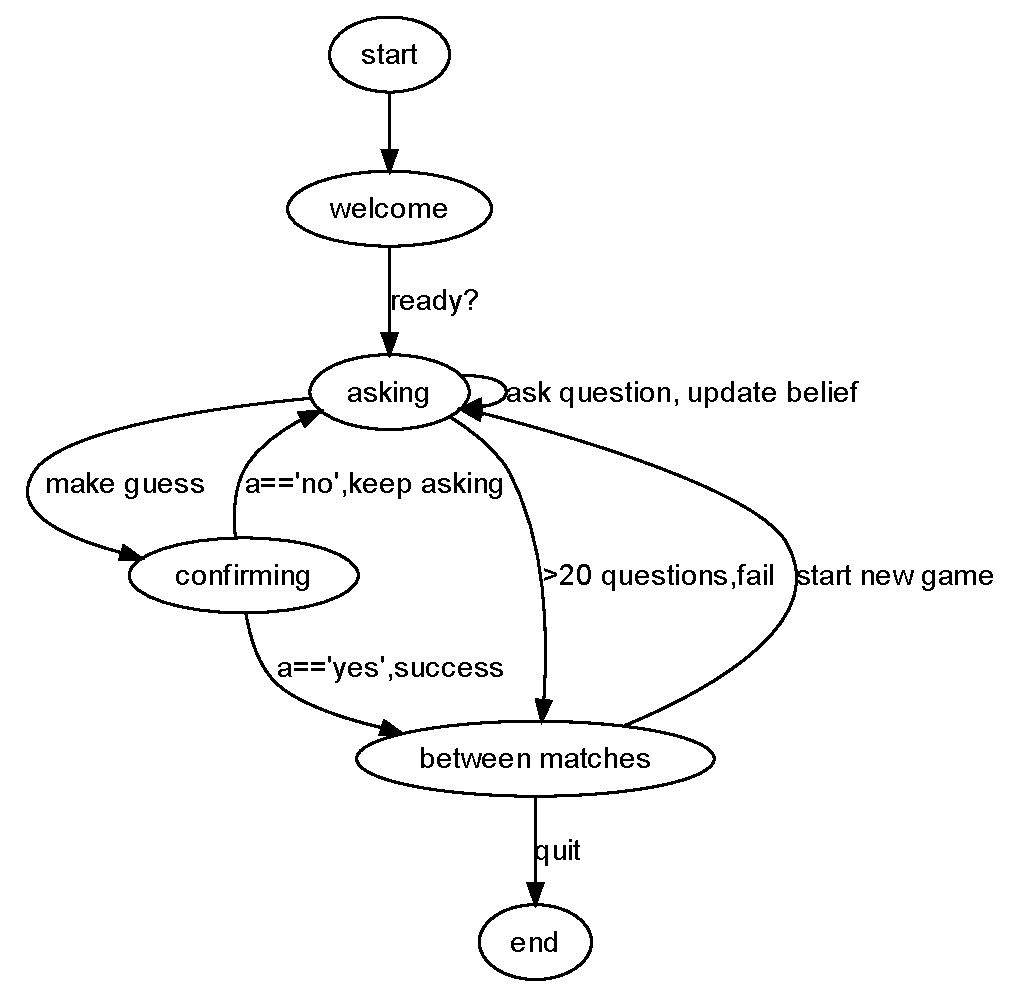
\includegraphics[scale=.45]{statemachine}
  %\vspace{-15pt}
  \caption{EMO20Q questioner agent state machine.}
  \label{statemachine}
  %\vspace{-14pt}

\end{figure}


%mention nltk and smoothing
%
%experimental validation

%\vspace{-10pt}

\section{Results}
\label{sec:results}



The results of our usability experiments on fifteen subjects are summarized in
Table \ref{tab:experimental-results} .  To compare the agent's performance
with human performance from previous studies \cite{Kazemzadeh2011a}, we used
two objective measures and one subjective measure. The success rate, shown in
column two Table \ref{tab:experimental-results}, is an objective measure of
how often the EMO20Q matches ended with the agent successfully guessing the
user's emotion.  The number of turns it took for the agent to guess the
emotion is the other objective measure.  The last column, naturalness, is a
subjective measure where users rated how human-like the agent was, on a 0-10
scale.

The emotion words chosen by the subjects as ``easy'' were recognized by the
agent with similar success rate and number of required turns as human-human
matches.  Some examples of ``easy'' emotions are anger, happiness, and
sadness. However, successful outcomes were fewer in emotions chosen as
``medium'' and ``difficult''.  Some examples of ``medium'' emotions are
contentment, curiosity, love, and tiredness. Pride, frustration,
vindication, and zealousness are examples of ``difficult'' emotions. The
different classes of words were not disjoint: some words like anger, disgust,
and confusion spanned several categories. A complete listing of the words chosen by the subjects of the experiment is given in Table \ref{tab:words}. 

The results in terms of successful outcomes and number of turns required to
guess the emotion word are roughly reflected in the percent of words that are
in vocabulary.  Despite the low performance on emotion words deemed ``medium''
and ``difficult'', there was not a corresponding decrease in the perceived
naturalness of the questioner agent.
%\vspace{-10pt}
\begin{table}[t]
\label{tab:experimental-results}
\caption{Experimental results.}
{\footnotesize
\begin{tabular}{|l|l|l|l|l|}
\hline
\textbf{difficulty} & \hspace{-3pt} \textbf{\% success}  & \hspace{-3pt}\textbf{avg. turns} & \hspace{-3pt}\textbf{\% in vocab.} & \hspace{-3pt}\textbf{naturalness} \\ \noalign{\hrule height 1pt}
easy       & 73\%       & 11.4       & 100\%        & 6.9 \\ 
medium     & 46\%       & 17.3       & 93\%         & 5.5 \\ 
difficult  & 13\%       & 18.2       & 60\%         & 5.8 \\ 
\hline
total      & 44\%     & 15.6  & 84\%  & 6.1 \\ 
\hline
\end{tabular}
}
%\vspace{-14pt}

\end{table}
% R commands

%> t <- read.csv("experiment.txt")
%> outcome <- t$success==1
%> t$outcome <- factor(outcome, levels=c(TRUE,FALSE), labels=c("success","failure"))

%> prop.table( table(t$outcome, factor(t$difficulty,levels=c("easy","medium","difficult"))),2)
%               easy    medium difficult                                        
%                success 0.8333333 0.5000000 0.0000000
%                failure 0.1666667 0.5000000 1.0000000                                                      
%> mean( t$turns)
% [1] 16.83333
% > mean( subset(t$turns,t$difficulty=="easy"))
% [1] 10.66667
%> mean( subset(t$turns,t$difficulty=="medium"))
% [1] 19.83333
%> mean( subset(t$turns,t$difficulty=="difficult"))
% [1] 20

%> prop.table(table(t$outcome))
%
%  success   failure
%  0.4444444 0.5555556

%> prop.table( table( factor(t$difficulty,levels=c("easy","medium","difficult")),factor(t$invocab,levels=c(1,0))),1)
%
%                    1         0
%  easy      1.0000000 0.0000000
%  medium    0.8333333 0.1666667
%  difficult 0.3333333 0.6666667

% prop.table( table( factor(t$invocab,levels=c(1,0))))
%
%         1         0
% 0.7222222 0.2777778

% > mean( subset(t$natural,t$invocab==1))t$natural
% > mean( subset(t$natural,t$difficulty=="easy"))
% [1] 7.333333
% > mean( subset(t$natural,t$difficulty=="medium"))
% [1] 5.333333
% > mean( subset(t$natural,t$difficulty=="difficult"))
% [1] 6.833333
% > mean( t$natural)
% [1] 6.5

\begin{table}
\label{tab:words}
\caption{Observed emotion words by difficulty.}
\begin{tabularx}{\columnwidth}{ |l|X| }
  \hline
  \textbf{difficulty} & \textbf{examples}  \\
  \noalign{\hrule height 1pt}
  easy & happiness, anger, sadness, calm, confusion  \\
  \hline 
  medium  & anger, confusion, contentment, curiosity, depression, disgust, excitement, fear, hate, irritation, love, melancholy, sorrow, surprise, tiredness  \\
  \hline
  difficult  & devastation, disgust, ecstasy, ennui, frustration, guilt, hope, irritation, jealousy, morose, proud, remorse, vindication, zealousness  \\
  \hline
\end{tabularx}
\end{table}
\section{Discussion}
\label{sec:discussion}

The results we obtained show that this model provides an agent that users find
to be human-like despite having fewer successful outcomes than in human-human
matches.  The naturalness of the agent's behavior will make it useful as a
tool to obtain more ethnographic data about how people describe emotions.  The
out-of-vocabulary rate observed in Table \ref{tab:words} indicates that the
agent is useful for eliciting new emotion words. Collecting more data would
continue to improve the agent's coverage and performance.  Apart from
collecting more data, here are also algorithmic and practical improvements
that can be made.

Algorithmically, the area that we could improve the most is the selection of
the next question.  Currently, the naive Bayes assumption of independence
results in similar questions being asked, especially questions that are
semantically opposite (e.g., ``is it a positive emotion?'' and ``is it a
negative emotion?''), so incorporating semantic relations between features
will help. Also, the selection of the next question based on the maximum
probability of the answer being ``yes'' tends to ask the same questions in
each match.  This repetitive behavior is not ideal if the goal is to collect a
wide variety of human knowledge, so this is another area for improvement. In
an earlier paper \cite{Kazemzadeh2011b}, we describe a methodology for
exploring questions that are not well represented in the training data in
order to create an agent that is an effective learner.  Other possible
approaches include choosing questions that minimize the expected entropy of
the posterior \cite{Geman1993,Jedynak2012}.

Another algorithmic issue for future work is that the EMO20Q agent learns in
batch-mode, meaning that it will make the same mistakes in consecutive dialogs
unless there is an explicit retraining.  Moreover, our current algorithm does
not react differently to incongruous information.  Besides learning
statistically from new data, it would be ideal to learn more from data that
appears incongruous or salient. Another technical issue is the quantization of
answers into \{yes, no, other\} categories.  This is a coarse categorization,
but it helps to decrease sparsity in the feature space.  Having a continuous
or fuzzy scale between ``yes'' and ``no'' is an alternative representation
that could provide a more informative representation while also avoiding
sparsity issues.

One practical improvement is to remove turns from the training data that
contain anaphoric references.  Because the agent automatically selects turns
from previous human-human matches for use in human-computer matches based only
on questions and answers, there are anaphora which are unresolved that appear
as non sequiturs to the users.  The presence of these non sequiturs led to less
informative responses and (based on the user comments) led to lower
naturalness scores.

The collection and representation of world knowledge is frequently a
bottleneck in both artificial intelligence and natural language processing.
Designing agents that can automatically collect this information is therefore
an important possibility in overcoming these limitations.  Many times, the
world knowledge problem is posed as a task of collecting facts.  However,
natural language descriptions of emotions may vary between cultures and over
time.  Therefore, rather than collecting facts to form a fixed ontology, we
feel that the idea of ethnography is more applicable for this kind of
subjective cultural data.  The question-asking framework to do this has been
theoretically described as a Socratic epistemology \cite{Hintikka2007}.  The
quantitative, computational approach to social sciences that is enabled by
natural language processing and the prevalence of online communication can be
seen in emerging fields such as sentiment analysis and crowd-sourcing.

The emotions recognized by the EMO20Q questioner agent are more conceptual
than the typical emotion recognition task.  Being able to integrate
traditional emotion recognition, i.e., the recognition of social signals, with
the understanding of natural language descriptions of emotions is an open issue
with many implications.  The task of annotation of emotional data is one area
where applying linguistic descriptions to emotions in social interactions
could be fruitful.  The same agent playing the role of an interlocutor as well
as an evaluator is an intriguing and important possibility with practical
applications to more ecologically-valid interaction based evaluation and
derivation of human informatics for clinicians and other analysts
\cite{Alderson-Day2011}.


The code and data for the agent described in this paper can be found at http://sail.usc.edu/emo20q .

%\vspace{-10pt}

\section{Acknowledgments}

%\vspace{-5pt}

The authors would like to thank the EMO20Q players, Nassos Katsamanis, Kartik
Audhkhasi, Jeremy Chi-Chun Lee, the reviewers of ACII2011, Ben Alderson-Day,
and Carbon Five Hack Night.

%\vspace{-5pt}

\eightpt
\bibliographystyle{IEEEtran}
%\bibliography{IEEEexample}
\bibliography{emo20q_naive_bayes.bib}

\end{document}
